\documentclass[border=2pt]{standalone}
\usepackage{tikz}
\usetikzlibrary{arrows.meta,positioning,calc,fit,backgrounds,shapes.geometric}
\usepackage{amsmath,amssymb}
\usepackage{times}
\definecolor{ink}{HTML}{243447}
\definecolor{cA}{HTML}{4477AA}
\definecolor{cB}{HTML}{CC6677}
\definecolor{cAu}{HTML}{44AA99}
\definecolor{cS}{HTML}{CCAA33}
\definecolor{grn}{HTML}{228833}
\definecolor{rose}{HTML}{AA3377}
\definecolor{inst}{HTML}{F2E3B3}
\tikzset{
 pap/.style={circle,draw=ink,line width=.6pt,minimum size=15pt,inner sep=0pt,font=\scriptsize\bfseries,text=white},
 aut/.style={rectangle,draw=ink,line width=.6pt,minimum size=13pt,inner sep=0pt,fill=cAu,font=\scriptsize\bfseries,text=white},
 sub/.style={diamond,draw=ink,line width=.6pt,minimum size=17pt,inner sep=0pt,fill=cS,font=\scriptsize\bfseries,text=white},
 gone/.style={draw=ink!35,fill=ink!8,text=ink!40,dashed},
 ed/.style={draw=ink,line width=.7pt},
 msg/.style={-{Stealth[length=4pt]},line width=.9pt,draw=rose},
 ptitle/.style={font=\footnotesize\bfseries,text=ink,anchor=west},
 note/.style={font=\scriptsize,text=ink,align=center},
}

\tikzset{
 est/.style={rectangle,draw=grn,fill=grn!15,line width=.5pt,minimum size=5pt,inner sep=0pt},
 fst/.style={circle,fill=rose,inner sep=1.5pt},
 tie/.style={line width=.75pt,draw=rose,{Stealth[length=3.5pt]}-{Stealth[length=3.5pt]}},
}
\begin{document}
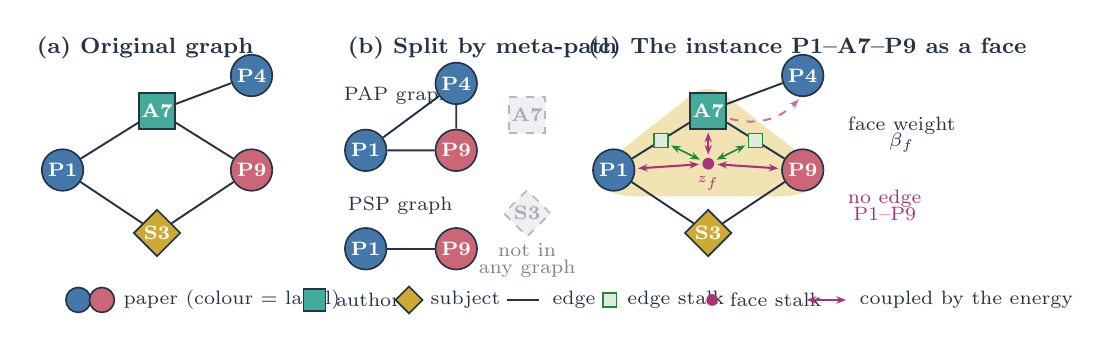
\begin{tikzpicture}
% ---------- (a) original graph
\begin{scope}[shift={(0,0)}]
\node[ptitle] at (-0.45,1.55) {(a) Original graph};
\node[pap,fill=cA] (P1) at (0,0) {P1};
\node[aut] (A7) at (1.2,0.75) {A7};
\node[sub] (S3) at (1.2,-0.8) {S3};
\node[pap,fill=cB] (P9) at (2.4,0) {P9};
\node[pap,fill=cA] (P4) at (2.4,1.2) {P4};
\draw[ed] (P1)--(A7) (A7)--(P9) (A7)--(P4) (P1)--(S3) (S3)--(P9);
\end{scope}
% ---------- (b) split by meta-path
\begin{scope}[shift={(3.85,0)}]
\node[ptitle] at (-0.35,1.55) {(b) Split by meta-path};
\node[note,anchor=west] at (-0.4,0.95) {PAP graph};
\node[pap,fill=cA] (bP1) at (0,0.25) {P1};
\node[pap,fill=cB] (bP9) at (1.15,0.25) {P9};
\node[pap,fill=cA] (bP4) at (1.15,1.1) {P4};
\draw[ed] (bP1)--(bP9) (bP1)--(bP4) (bP4)--(bP9);
\node[note,anchor=west] at (-0.35,-0.45) {PSP graph};
\node[pap,fill=cA] (cP1) at (0,-1.0) {P1};
\node[pap,fill=cB] (cP9) at (1.15,-1.0) {P9};
\draw[ed] (cP1)--(cP9);
\node[aut,gone] (gA) at (2.05,0.7) {A7};
\node[sub,gone] (gS) at (2.05,-0.55) {S3};
\node[note,text=ink!60] at (2.05,-1.15) {not in\\[-2pt]any graph};
\end{scope}
% ---------- (c) ours: the instance as a face
\begin{scope}[shift={(7.0,0)}]
\node[ptitle] at (-0.45,1.55) {(c) The instance P1--A7--P9 as a face};
\node[pap,fill=cA] (oP1) at (0,0) {P1};
\node[aut] (oA7) at (1.2,0.75) {A7};
\node[sub] (oS3) at (1.2,-0.8) {S3};
\node[pap,fill=cB] (oP9) at (2.4,0) {P9};
\node[pap,fill=cA] (oP4) at (2.4,1.2) {P4};
\begin{scope}[on background layer]
\fill[inst,rounded corners=7pt] ($(oP1.west)+(-0.08,-0.1)$) -- ($(oA7.north)+(0,0.13)$) -- ($(oP9.east)+(0.08,-0.1)$) -- ($(oP9.south)+(0,-0.06)$)--($(oP1.south)+(0,-0.06)$) -- cycle;
\end{scope}
\draw[ed] (oP1)--(oA7) (oA7)--(oP9) (oA7)--(oP4) (oP1)--(oS3) (oS3)--(oP9);
% edge stalks on the two edges of the face
\node[est] (s0) at ($(oP1)!0.5!(oA7)$) {};
\node[est] (s1) at ($(oA7)!0.5!(oP9)$) {};
% face stalk
\node[fst] (zf) at (1.2,0.08) {};
\node[note,text=rose,font=\tiny] at (1.2,-0.17) {$z_f$};
\draw[tie,shorten <=1pt,shorten >=1pt] (zf) -- (oP1);
\draw[tie,shorten <=1pt,shorten >=1pt] (zf) -- (oP9);
\draw[tie,shorten <=1pt,shorten >=1pt] (zf) -- (oA7);
\draw[tie,draw=grn,line width=.6pt,shorten <=1pt,shorten >=1pt] (zf) -- (s0);
\draw[tie,draw=grn,line width=.6pt,shorten <=1pt,shorten >=1pt] (zf) -- (s1);
\draw[-{Stealth[length=3.5pt]},line width=.7pt,draw=rose!70,dashed] ($(oA7.east)+(0.04,-0.1)$) to[bend right=30] ($(oP4.south)+(-0.05,-0.03)$);
\node[note,anchor=west] at (2.85,0.45) {face weight\\[-2pt]$\beta_f$};
\node[note,anchor=west,text=rose] at (2.85,-0.45) {no edge\\[-2pt]P1--P9};
\end{scope}
% legend
\begin{scope}[shift={(0.2,-1.65)}]
\node[pap,fill=cA,minimum size=9pt] (l1) at (0,0) {}; \node[pap,fill=cB,minimum size=9pt] (l1b) at (0.3,0) {};
\node[note,anchor=west] at (0.45,0) {paper (colour = label)};
\node[aut,minimum size=8pt] at (3.0,0) {}; \node[note,anchor=west] at (3.15,0) {author};
\node[sub,minimum size=10pt] at (4.2,0) {}; \node[note,anchor=west] at (4.35,0) {subject};
\draw[ed] (5.45,0)--(5.85,0); \node[note,anchor=west] at (5.9,0) {edge};
\node[est] at (6.75,0) {}; \node[note,anchor=west] at (6.85,0) {edge stalk};
\node[fst] at (8.05,0) {}; \node[note,anchor=west] at (8.15,0) {face stalk};
\draw[tie] (9.25,0)--(9.75,0); \node[note,anchor=west] at (9.8,0) {coupled by the energy};
\end{scope}
\end{tikzpicture}
\end{document}
